% This is a sample document using the University of Minnesota, Morris, Computer Science
% Senior Seminar modification of the ACM sig-alternate style. Much of this content is taken
% directly from the ACM sample document illustrating the use of the sig-alternate class. Certain
% parts that we never use have been removed to simplify the example, and a few additional
% components have been added.

% See https://github.com/UMM-CSci/Senior_seminar_templates for more info and to make
% suggestions and corrections.

\documentclass{sig-alternate}
\usepackage{color}
\usepackage[colorinlistoftodos]{todonotes}

%%%%% Uncomment the following line and comment out the previous one
%%%%% to remove all comments
%%%%% NOTE: comments still occupy a line even if invisible;
%%%%% Don't write them as a separate paragraph
%\newcommand{\mycomment}[1]{}

\begin{document}

% --- Author Metadata here ---
%%% REMEMBER TO CHANGE THE SEMESTER AND YEAR AS NEEDED
\conferenceinfo{UMM CSci Senior Seminar Conference, December 2017}{Morris, MN}

\title{Point-of-Interest Recommendation Systems in Location-Based Social Networks}

\numberofauthors{1}

\author{
% The command \alignauthor (no curly braces needed) should
% precede each author name, affiliation/snail-mail address and
% e-mail address. Additionally, tag each line of
% affiliation/address with \affaddr, and tag the
% e-mail address with \email.
\alignauthor
Myeongjae Song\\
	\affaddr{Division of Science and Mathematics}\\
	\affaddr{University of Minnesota, Morris}\\
	\affaddr{Morris, Minnesota, USA 56267}\\
	\email{songx823@morris.umn.edu}
}

\maketitle
\begin{abstract}
``TBA"
\emph{This will be gone (hopefully)}

% The current paper format *only* allows inline comments using the todo
% macro. That's kind of a bummer, and it would be neat if someone figured
% out how to change the acmconf style to allow this. I suspect it isn't *hard*
% but there are quite a few details that have to be sorted out in synchrony.
\todo[inline]{Needs more work}
\end{abstract}

\keywords{Recommendation Systems, Point-of-Interest Recommendation, Location-Based Social Networks}

\section{Introduction}
\label{sec:introduction}

Nowadays, location-based social networks (LBSN), such as \emph{Facebook places, Tinder},  and \emph{Yelp}, 
have been gaining a lot of attention with the widespread use of smartphones embedded with the 
global positioning system (GPS). Even though LBSN are relatively new compared to 
the traditional social networking services, millions of active users use the platform on a daily basis voluntarily sharing 
their location information. Many of these LBSN allow users to ``check-in" 
places like a restaurant or cinema; we call these checked-in places the points of interests (POI) 
of the users. Users can share videos, pictures, or reviews about the places via this ``check-in" 
feature. Based on the collected user data, LBSN provide POI recommendations. POI recommendation 
is very important for LBSN for two reasons. First, users are more likely use the platform and check-in places 
for their own benefits if it gives accurate predictions on places where users visit next. 
Second, it allows the advertisers launch advertisements for target user group. Therefore, 
accurate POI recommendation is crucial for the success of LBSN.

Even though POI recommendation is a type of recommendation system, it has distinct characteristics 
mainly due to its geographical nature. For instance, recommending a movie is a fairly different task from 
recommending a place. A movie recommendation system can recommend any movie, but a POI recommendation 
system cannot just recommend a sushi restaurant in Tokyo for a user in Minnesota. The following are 
meaningful differences between conventional recommendations and POI recommendation:

\begin{itemize}
\item[--] The types of checked-in place are highly related to the time period. Figure 1 shows check-in data in 
NYC from a LBSN (Foursquare) over different hours of a day. The number of check-ins clearly varies depending 
on the time.
\item[--] People are likely to visit nearby places because of geographical limitation. Not many people are willing 
to fly to Japan from the US just for a nice sushi restaurant.
\item[--] The transition between POI is strongly affected by the user's own preference. Li et al. [2017] refers this as a long-term individual preference. For instance, some people go to the gym after work, but some people go home right away after work. 
\item[--] User's next location is highly related to the user's current location. We would call this sequential feature of POI recommendation. 
\end{itemize}

Traditionally, matrix factorization (MF) or Markov chain (MC) have been popular techniques for producing recommendations. 
Because of the known drawbacks of each model, Rendle et al. [2010] proposes factorizing personalized 
Markov chains (FPMC), which the combination of MC and MF techniques. FPMC is a robust system, 
but it is a genetic model and not designed for POI recommendations. To capture the locality feature of 
POI recommendations, Cheng et al. [2013] suggests FPMC-LR method. And, Li et al. [2017] proposes 
TAD-FPMC, which is an improvement over FPMC-LR.

In section 2, we are going to cover general and mathematical backgrounds in recommendation systems 
to understand the proposed models. Then in section 3, we will explore the proposed approaches in detail. 
In section 4, we will compare the accuracy of different recommendation techniques: FPMC, FPMC-LR, and TAD-FPMC. 
Finally, we will conclude the paper in section 5.

\section{Backgrounds}
\label{sec:backgrounds}

TBA

\section{Factoring Personalized Markov Chain and its improvements}
\label{sec:fpmc}

As we have discussed in section \ref{sec:backgrounds}, MC and MF based recommender systems
have fairly distinct characteristics from each other. In this section, we will study a model called 
Factoring Personalized Markov Chain (FPMC) that incorporates MF into MC, and then its 
enhancements specializing in LSBN data properties.

\subsection{Formalizaion}
\label{sec:typeChangesSpecialChars}

Before we dive into the details, let us introduce the notation used in this paper. 
Let $U$ be a set of users and $L$ be a set of locations. For each user $u$ in $U$, 
we know their check-in history set \begin{math}L^t_u\end{math} where $t$ is a timestamp 
of the user visit. Our goal now is given the user check-in data 
\begin{math}L^1_u,...,L^t_u\end{math}, recommend a next location to 
a user $u$ at time $t + 1$.

\subsection{FPMC}
\label{sec:typeChangesSpecialChars}

Even though MC based recommender systems were widely studied and used because of 
its capacity to capture sequential data, it lacks the personalization feature to distinguish each user. 
MF also has its weakness in processing sequential information since it is often completely ignored 
to focus on the general taste of each user. The weakness is particularly problematic in LBSN. 
In LBSN, sequential information plays a huge role in that there is a strong connection 
between recently visited locations and future locations. For instance, people are likely to visit 
cinemas or bars after restaurants. However, a recommender system with no sequential awareness 
may recommend another restaurant to a user who just check-ined a restaurant; this is not ideal. 
To take advantage of both MF and MC models, Rendle et al. [2010] proposes factorizing personalized 
Markov chains (FPMC).

How does FPMC combine these two different techniques? The most straightforward solution that 
we can think of is having a personalized MC per user. Figure 3 shows four different transition matrices for each user. 
? entries mean we have no data 
to estimate the probability of the transition. As we can observe from the matrices, simply using 
personalized transition matrices produces poor estimations. We just do not have enough data from
each user. This is the place where the ideas of 
MF can be applied. By stacking all transition matrices of users, we can get a transition cube or tensor A. 
This is the essence of FPMC. Figure 4 represents the tensor for the same data from figure 3. 
Unlike the naive personalization MC approach, a factored tensor solves the sparsity problem and 
still has its personalization feature for individual users.

\begin{figure}
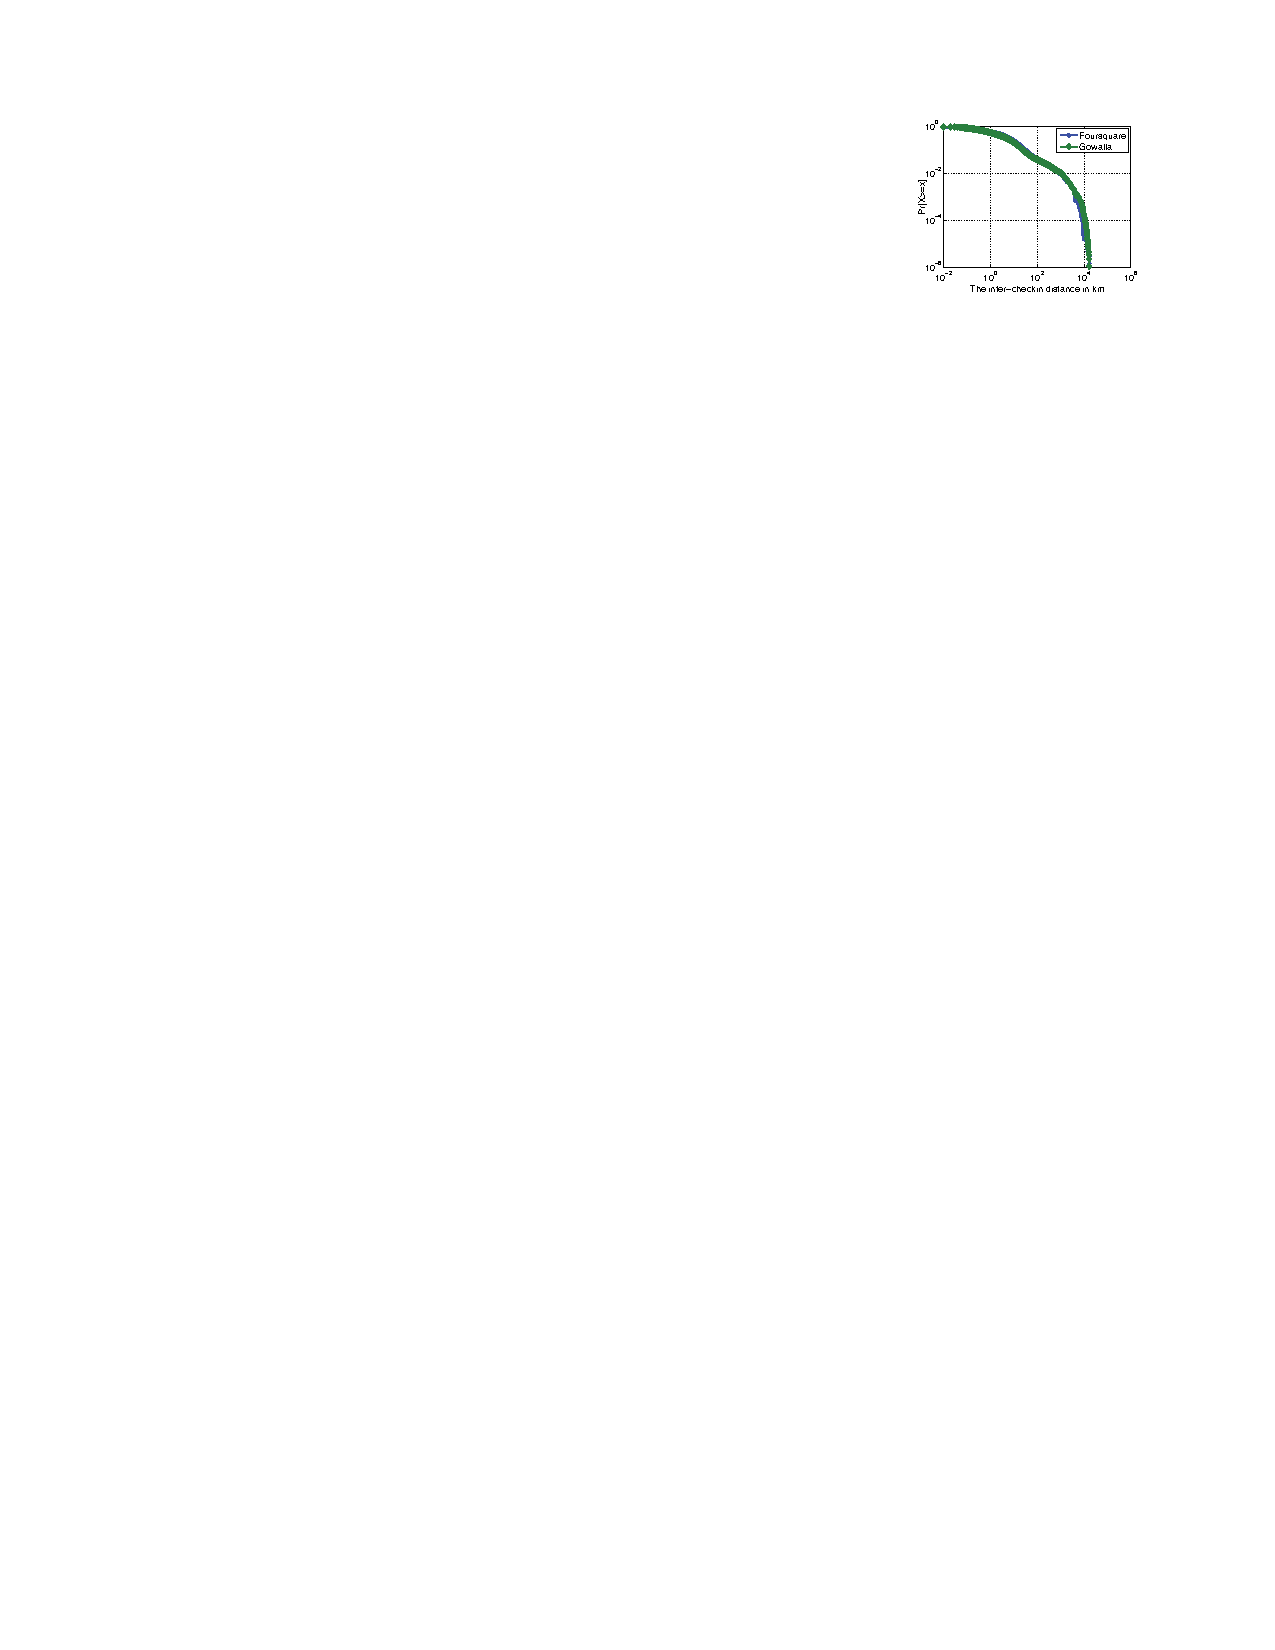
\psfig{file=Figure4(b).pdf,width=3in}
\caption{The inter check-in distance in km}
\label{fig:onlyOne}
\end{figure}

\subsection{FPMC-LR}
\label{sec:typeChangesSpecialChars}

FPMC successfully incorporates the information of the personalized Markov chain 
by combining MF and MC in CF. However, it overlooks another noticeable property 
of the LBSN datasets, localized region constraint. The figure ~\ref{fig:onlyOne}  
reports the distance of inter check-ins in Gowalla and Foursquare. It shows that 
more than 75\% of inter check-ins from Foursquare and 80\% of inter check-ins 
from Gowalla happened within 10 km. Only less than 5\% of inter check-ins occur 
more than 100km both in Foursquare and Gowalla. The observation on the LBSN 
shows the trend that users tend to check in places close to their previous check-ins, 
but the FPMC does not really make use of this potentially useful trend.

(Intro to FPMC-LR non-tech) To add the ability to use localized region constraint 
information into the existing personalized POI Markov chain, Cheng et al. [2013] 
introduces a model called FPMC-LR which combines FPMC model with localized 
region constraints to provide accurate successive POI recommendation in LBSNs. 
Because FPMC-LR only takes into account nearby candidate locations depending 
on where the users are, it reduces the computational costs and noisy information. 
Also, it results in more accurate predications as we will see in [section result].

(Math part) FPMC-LR model has a similar setting as FPMC since it is an improvement 
over it. Just like in FPMC, the fundamental goal of FPMC-LR is to give the most suitable 
location recommendation for user $u$ at time $t + 1$, given a sequence of check-ins. 
In other words, we need to calculate the probability of a user $u$ to visit a location $l$ at time $t$:
\begin{equation}
	x_{u,i,l}=p(l \in L_u^t | i \in L_u^{t-1})
\label{eq:summation}
\end{equation}
The main difference between FPMC and FPMC-LR is in their transition tensor. As we saw earlier, in FPMC, the model takes into account all possible locations for each user, so the tensor looks like: 
\begin{equation}
	\chi \in [0, 1]^{|U| \times |L| \times |L|}
\label{eq:summation}
\end{equation}
In FPMC-LR, the model only considers neighbor locations for each location l for each user. 
The tensor transition in FPMC-LR looks like:
\begin{equation}
	\chi \in [0, 1]^{|U| \times |L| \times |N_d(L)|}
\label{eq:summation}
\end{equation}
The neighbor locations \begin{math}N_d(L)\end{math} are calculated by Haversine formula, 
which is used to find the shortest distance between two points on the surface of a sphere. 
In this case, we assume the earth is a roughly sphere. After applying several steps of ranking techniques, 
we can get the final probability \begin{math}x_u,t,l\end{math}.

\subsection{TAD-FPMC}
\label{sec:typeChangesSpecialChars}

FPMC-LR is a very successful model for POI recommendation in terms of performance and efficiency 
as we will discuss in later section; it incorporates sequential data with personalization and locality consideration. 
However, there is a still room for improvement. Li et al. [2017] points out that FPMC-LR approach simply captures 
the consecutive ordering relations in lieu of considering complex user behavior over time. Take college students, 
for example. Students have morning classes, afternoon classes, or both in one day. When they have morning classes, 
some of them have breakfast at a brunch café after class. When they have afternoon classes, some of them go 
for a drink at a bar. Simply combining them as one sequential pattern is clearly not sufficient (e.x. recommending 
for a drink at a bar after 8:00AM class). In other words, just recognizing sequential data such as the pattern is not 
enough for capturing the differences in regular periodic pattern.

To make the system consider time-varying behavioral trends, Li et al. [2017] suggests time-aware FPMC (TA-FPMC) 
model, which is an improvement over FPMC-LR model. In section 2-1, Rendle et al. [2010] uses third order tensor to 
construct a personalized Markov chain. TA-FPMC takes a similar approach. Instead of a third order tensor of 
user-location-location, it forms a fourth order tensor by adding a time factor. Now, the transition tensor looks like: 
There is another statistical characteristic of LBSN data that has not got much attention, the time gap between 
two successive check-ins. The LBSN data shows that many of two successive check-ins span a large time gap 
like a year. Base on the assumption that these successive check-ins with large time gaps do not tell much, 
Li et al. [2017] introduces another factor D(delta t) to take into account the time-decaying effect. 
The final model with all the considerations is called TAD-FPMC.


\section{Body}
\label{sec:body}

Typically, the body of a paper is organized
into a hierarchical structure, with numbered or unnumbered
headings for sections, subsections, sub-subsections, and even
smaller sections.  The command \texttt{\textbackslash section} that
precedes this paragraph is part of such a
hierarchy.\footnote{This is the second footnote.  It
starts a series of three footnotes that add nothing
informational, but just give an idea of how footnotes work
and look. It is a wordy one, just so you see
how a longish one plays out.} \LaTeX\ handles the numbering
and placement of these headings for you, when you use
the appropriate heading commands around the titles
of the headings.  If you want a sub-subsection or
smaller part to be unnumbered in your output, simply append an
asterisk to the command name.  Examples of both
numbered and unnumbered headings will appear throughout the
balance of this sample document.

Because the entire article is contained in
the \textbf{document} environment, you can indicate the
start of a new paragraph with a blank line in your
input file; that is why this sentence forms a separate paragraph.

\subsection{Type Changes and {\subsecit Special} Characters}
\label{sec:typeChangesSpecialChars}

We have already seen several typeface changes in this sample.  You
can indicate italicized words or phrases in your text with
the command \texttt{\textbackslash textit}; emboldening with the
command \texttt{\textbackslash textbf}
and typewriter-style (for instance, for computer code) with
\texttt{\textbackslash texttt}.
As a rule you'd prefer \texttt{\textbackslash emph} (which stands for \emph{emphasize})
over something like \texttt{\textbackslash textit} since that gives the typesetting system
more flexibility in how it can emphasize that text.

You do not
have to indicate typestyle changes when such changes are
part of the \textit{structural} elements of your
article; for instance, the heading of this subsection will
be in a sans serif\footnote{A third footnote, here.
Let's make this a rather short one to
see how it looks.} typeface, but that is handled by the
document class file. Take care with the use
of\footnote{A fourth, and last, footnote.}
the curly braces in typeface changes; they mark
the beginning and end of
the text that is to be in the different typeface.

You can use whatever symbols, accented characters, or
non-English characters you need anywhere in your document;
you can find a complete list of what is
available in the \textit{\LaTeX\
User's Guide}~\cite{Lamport:LaTeX}.

\subsection{Math Equations}
\label{sec:mathEquations}

You may want to display math equations in three distinct styles:
inline, numbered or non-numbered display.  Each of
the three are discussed in the next sections.

\subsubsection{Inline (In-text) Equations}
\label{sec:inlineEquations}

A formula that appears in the running text is called an
inline or in-text formula.  It is produced by the
\textbf{math} environment, which can be
invoked with the usual \texttt{\textbackslash begin\ldots\textbackslash end}
construction or with the short form \texttt{\$\ldots \$}. You
can use any of the symbols and structures,
from $\alpha$ to $\omega$, available in
\LaTeX~\cite{Lamport:LaTeX}; this section will simply show a
few examples of in-text equations in context. Notice how
this equation: \begin{math}\lim_{n\rightarrow \infty}x=0\end{math},
set here in in-line math style, looks slightly different when
set in display style.  (See next section).

\subsubsection{Display Equations}
\label{sec:displayEquations}

A numbered display equation -- one set off by vertical space
from the text and centered horizontally -- is produced
by the \textbf{equation} environment. An unnumbered display
equation is produced by the \textbf{displaymath} environment.

Again, in either environment, you can use any of the symbols
and structures available in \LaTeX; this section will just
give a couple of examples of display equations in context.
First, consider the equation, shown as an inline equation above:

\begin{equation*}
\lim_{n\rightarrow \infty}x=0
\end{equation*}

Notice how it is formatted somewhat differently in
the \textbf{displaymath}
environment.  Now, we'll enter an unnumbered equation:

\begin{displaymath}
	\sum_{i=0}^{\infty} x + 1
\end{displaymath}

and follow it with a numbered equation (Equation~\ref{eq:summation}):

\begin{equation}
	\sum_{i=0}^{\infty}x_i=\int_{0}^{\pi+2} f
\label{eq:summation}
\end{equation}

just to demonstrate \LaTeX's able handling of numbering.
Note that if you use numbered equations, you can give them \texttt{label}s
and \texttt{\textbackslash ref} them, e.g., Equation~\ref{eq:summation}.

\subsection{Multi-line formulas}
\label{sec:multiLineFormulas}

The \texttt{align} and \texttt{align*} environments let you align sequences of
equations so, for examples, a sequences of equal signs line up nicely. 

% The & creates a "virtual tab stop" and corresponding &'s on each line
% will be aligned when the layout is done.
\begin{align*}
n_1 &= \sum_{i = 1}^k a_i \\
n_{x-y} &= \prod_{i = 1}^k b_i
\end{align*}

\begin{align*}
 f(x) &= (x+a)(x+b) \\
 &= x^2 + (a+b)x + ab
\end{align*}

\subsection{Figures}
\label{sec:figures}

Like tables, figures cannot be split across pages; the
best placement for them
is typically the top or the bottom of the page nearest
their initial cite.  To ensure this proper ``floating'' placement
of figures, use the environment
\textbf{figure} to enclose the figure and its caption.

This sample document contains examples of
a \textbf{.pdf} file to be displayable with \LaTeX, such as
Figure~\ref{fig:singleColumnFigure}.  More
details on each of these is found in the \textit{Author's Guide}.

\begin{figure}
\centering
\psfig{file=sample_graph.pdf,width =3in}
\caption{A sample graph just spanning one column.}
\label{fig:singleColumnFigure}
\end{figure}


As was the case with tables, you may want a figure
that spans two columns, like Figure~\ref{fig:twoColumnFigure}.  
To do this, and still to
ensure proper ``floating'' placement of tables, use the environment
\texttt{figure*} to enclose the figure and its caption.
And don't forget to end the environment with
\texttt{figure*}, not \texttt{figure}!

\begin{figure*}
\centering
\psfig{file=sample_graph.pdf,width =5.3in}
\caption{A sample graph that needs to span two columns of text.}
\label{fig:twoColumnFigure}
\end{figure*}

It's easiest and you tend to get the best quality if your figure uses vector graphics
in PDF format. You can include other formats such as PNG, but they will usually
not look nearly as professional, especially when printed on high resolution printers.
\emph{Be very wary of screen captures from other papers. They tend to look pixelated
and amateurish even at high resolutions.}

\subsection{Tables}
\label{sec:tables}

Because tables cannot be split across pages, the best
placement for them is typically the top of the page
nearest their initial cite.  To
ensure this proper ``floating'' placement of tables, use the
environment \textbf{table} to enclose the table's contents and
the table caption.  The contents of the table itself must go
in the \textbf{tabular} environment, to
be aligned properly in rows and columns, with the desired
horizontal and vertical rules.  Again, detailed instructions
on \textbf{tabular} material
is found in the \textit{\LaTeX\ User's Guide}.

Immediately following this sentence is the point at which
Table~\ref{tab:frequencyOfSpecialChars} is included in the input file; 
compare the placement of the table here with the table in the
PDF output running \LaTeX\ on this document.

\begin{table}[t]
\centering
\caption{Frequency of Special Characters}
\label{tab:frequencyOfSpecialChars}
\begin{tabular}{c|c|l}
Non-English or Math & Frequency & Comments\\ \hline
\O & 1 in 1,000 & For Swedish names\\
$\pi$ & 1 in 5 & Common in math\\
\$ & 4 in 5 & Used in business\\
$\Psi^2_1$ & 1 in 40,000 & Unexplained usage\\
\end{tabular}
\end{table}

To set a wider table, which takes up the whole width of
the page's live area, use the environment
\textbf{table*} to enclose the table's contents and
the table caption, as demonstrated in Table~\ref{tab:typicalCommands} below.  
As with a single-column table, this wide
table will ``float" to a location deemed more desirable.
Immediately following this sentence is the point at which
Table~\ref{tab:typicalCommands} is included in the input file; again, it is
instructive to compare the placement of the
table here with the table in the printed dvi
output of this document.


\begin{table*}[t]
\centering
\caption{Some Typical Commands}
\label{tab:typicalCommands}
\begin{tabular}{ccl}
Command & A Number & Comments \\ \hline
\texttt{\textbackslash alignauthor}     & 100 & Author alignment\\
\texttt{\textbackslash numberofauthors} & 200 & Author enumeration\\
\texttt{\textbackslash table}           & 300 & For tables\\
\texttt{\textbackslash table*}          & 400 & For wider tables\\ 
\end{tabular}
\end{table*}
% end the environment with {table*}, NOTE not {table}!

\subsection{Citations}
\label{sec:citations}

Citations to articles~\cite{Aaronson:2005,Garey:1979,Brun:2008} listed
in the Bibliography section of your
article will occur throughout the text of your article.
You should use BibTeX to automatically produce this bibliography;
you simply need to insert one of several citation commands with
a key of the item cited in the proper location in
the \texttt{.tex} file~\cite{OM:2008}.
The key is a short reference you invent to uniquely
identify each work; in this sample document, the key is
the first author's surname and a
word from the title.  This identifying key is included
with each item in the \texttt{.bib} file for your article.

It is recommended that you precede \texttt{\textbackslash cite} (and 
\texttt{\textbackslash ref}) commands with a tilde
character instead of a space, e.g., \texttt{some text\textasciitilde\textbackslash cite}. The tilde gives you a non-breaking space which ensures that your citation won't get
stranded by itself on the beginning of a line.

The details of the construction of the \texttt{.bib} file
are beyond the scope of this sample document, but more
information can be found in the \textit{Author's Guide},
and exhaustive details in the \textit{\LaTeX\ User's
Guide}.

This article shows only the plainest form
of the citation command, using \texttt{\textbackslash cite},
which is all that is needed for our senior seminar.
You shouldn't use any other forms here.

\subsection{Theorem-like Constructs}
\label{sec:theoremLikeConstructs}

Other common constructs that may occur in your article are
the forms for logical constructs like theorems, axioms,
corollaries and proofs.  There are
two forms, one produced by the
command \texttt{\textbackslash newtheorem} and the
other by the command \texttt{\textbackslash newdef}; perhaps
the clearest and easiest way to distinguish them is
to compare the two in the output of this sample document:

Theorem~\ref{thm:integration} below uses the \textbf{theorem} environment, created by
the \texttt{\textbackslash newtheorem} command:

% You would usually put a \newtheorem command up at the top 
% of your LaTeX document after the \usepackage commands. It's
% just here in this example so it's with the text that describes it.
\newtheorem{theorem}{Theorem}

\begin{theorem}
Let $f$ be continuous on $[a,b]$.  If $G$ is
an antiderivative for $f$ on $[a,b]$, then
\begin{displaymath}\int^b_af(t)dt = G(b) - G(a).\end{displaymath}
\label{thm:integration}
\end{theorem}

The other uses the \textbf{definition} environment, created
by the \texttt{\textbackslash newdef} command:
\newdef{definition}{Definition}
\begin{definition}
If $z$ is irrational, then by $e^z$ we mean the
unique number which has
logarithm $z$: \begin{displaymath}{\log e^z = z}\end{displaymath}
\end{definition}

Two lists of constructs that use one of these
forms is given in the
\textit{Author's  Guidelines}.
 
There is one other similar construct environment, which is
already set up
for you; i.e. you must \textit{not} use
a \texttt{\textbackslash newdef} command to
create it: the \textbf{proof} environment.  Here
is a example of its use:
\begin{proof}
Suppose on the contrary there exists a real number $L$ such that
\begin{displaymath}
\lim_{x\rightarrow\infty} \frac{f(x)}{g(x)} = L.
\end{displaymath}
Then
\begin{align*}
l &= \lim_{x\rightarrow c} f(x) \\
  &= \lim_{x\rightarrow c}
\left[ g{x} \cdot \frac{f(x)}{g(x)} \right ] \\
  &= \lim_{x\rightarrow c} g(x) \cdot \lim_{x\rightarrow c}
\frac{f(x)}{g(x)}  \\
  &= 0\cdot L  \\
  &= 0,
\end{align*}
which contradicts our assumption that $l\neq 0$.
\end{proof}

Complete rules about using these environments and using the
two different creation commands are in the
\textit{Author's Guide}; please consult it for more
detailed instructions.  If you need to use another construct,
not listed therein, which you want to have the same
formatting as the Theorem
or the Definition~\cite{salas:calculus} shown above,
use the \texttt{\textbackslash newtheorem} or the
\texttt{\textbackslash newdef} command,
respectively, to create it.

\subsection*{A {\secit Caveat} for the \TeX\ Expert}
\label{sec:caveatForExperts}

Because you have just been given permission to
use the \texttt{\textbackslash newdef} command to create a
new form, you might think you can
use \TeX's \texttt{\textbackslash def} to create a
new command: \textit{Please refrain from doing this!}
Remember that your \LaTeX\ source code is primarily intended
to create camera-ready copy, but may be converted
to other forms -- e.g. HTML. If you inadvertently omit
some or all of the \texttt{\textbackslash def}s recompilation will
be, to say the least, problematic.

\section{Conclusions}
\label{sec:conclusions}

This paragraph will end the body of this sample document.
Remember that you might still have Acknowledgments or
Appendices; brief samples of these
follow.  There is still the Bibliography to deal with; and
we will make a disclaimer about that here: with the exception
of the reference to the \LaTeX\ book, the citations in
this paper are to articles which have nothing to
do with the present subject and are used as
examples only.

\section*{Acknowledgments}
\label{sec:acknowledgments}

This section is optional; it is a location for you
to acknowledge grants, funding, editing assistance and
what have you.

You want to use the \texttt{\textbackslash section*} version of the \texttt{section}
command, as an acknowledgments section typically does \emph{not} get
a number.

It is common (but by no means necessary) for students to thank
their advisor, and possibly other faculty, friends, and family who provided
useful feedback on the paper as it was being written.

In the present case, for example, the
authors would like to thank Gerald Murray of ACM for
his help in codifying this \textit{Author's Guide}
and the \textbf{.cls} and \textbf{.tex} files that it describes.

% The following two commands are all you need in the
% initial runs of your .tex file to
% produce the bibliography for the citations in your paper.
\bibliographystyle{abbrv}
% sample_paper.bib is the name of the BibTex file containing the
% bibliography entries. Note that you *don't* include the .bib ending here.
\bibliography{sample_paper}  
% You must have a proper ".bib" file
%  and remember to run:
% latex bibtex latex latex
% to resolve all references

\end{document}
